

For the programs of the same adaptivity complexity, we evaluate their average generalization error measured by root-mean-square error over fresh testing data.
Then with our tool, we choose different mechanism and evaluate each over the same data.
We plot the evaluation result in Figure~\ref{fig:implementation_generalization_errors}.
The result shows that for the same data analysis program, the generalization error is reduced
by equipping with the proper mechanism chosen by our model.




In Figure~\ref{fig:implementation_generalization_errors}(a), we plot the evaluation result over the
programs from the sklearn benchmark with $O(c)$ adaptivity.
We test them for classifying a randomly generated dataset with $n$ raw and $k$ features, and each raw is
assigned a random label from $\{-1, 1\}$.
We run these programs with constant number of adaptivity rounds and increasing the number of
maximum query numbers.
Then we evaluate the generalization error using underlying distribution that generate these data.
% from an underlying distribution


In Figure~\ref{fig:implementation_generalization_errors}(b), we plot the 
evaluation result over the fully adaptive
programs from the tensorflow benchmark with $O(n)$ adaptivity.
We evaluate these programs in the same way as the evaluation for the $O(c)$ adaptivity programs.
% for classifying a randomly generated dataset with $n$ raw and constant dimension.
% Then we evaluate the generalization error using underlying distribution that generate these data.

For these data analysis programs,
our tool is able to identify the $O(c)$ and $O(n)$ adaptivity level.
Then by choosing different mechanisms according to our tool,
the evaluation results show that the generalization error is reduced better than 
using the mechanisms without our tool.

In Figure~\ref{fig:implementation_generalization_errors}(c), we plot the 
evaluation result on
%  the over the
program implemented from~\cite{Jamieson2015TheAO} with $O(2^n)$ adaptivity.
We test this algorithm for ranking a random dataset. 
We run this algorithm over a randomly generated sample dataset with $n$ raw and constant dimension,
then we evaluate the generalization error for ranking
a fresh data generated under the same distribution.
We measure its root-mean-square error by counting the incorrectly ranked items.
For the data analysis with exponential adaptivity, our tool is able to identify the high adaptivity level.
Then by using the appropriate mechanism according to the adaptivity level,
the generalization error is reduced more than using other mechanisms.


{\small
\begin{figure}
\centering
\begin{subfigure}{.32\textwidth}
\begin{centering}
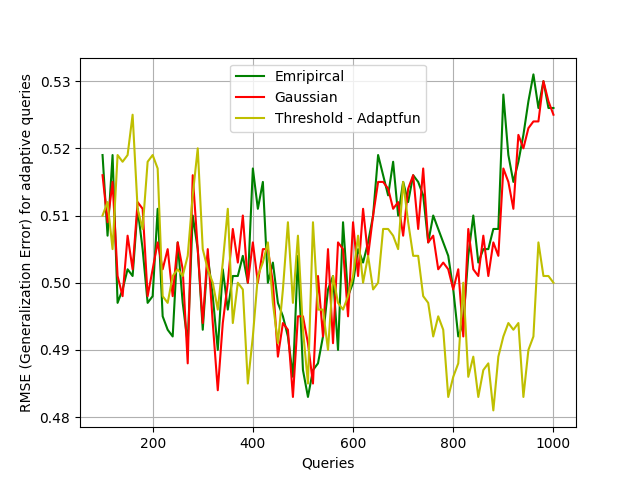
\includegraphics[width=1.0\textwidth]{c_adaptivity.png}
\caption{}
\end{centering}
\end{subfigure}
\begin{subfigure}{.32\textwidth}
\begin{centering}
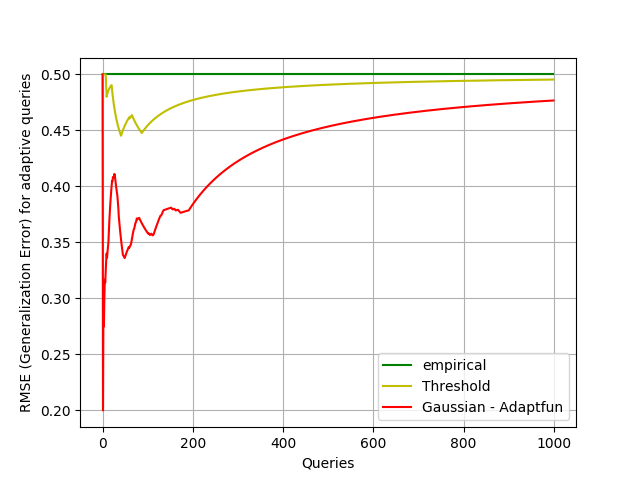
\includegraphics[width=1.0\textwidth]{n_adaptivity.png}
\caption{}
\end{centering}
\end{subfigure}
\quad
\begin{subfigure}{.3\textwidth}
\begin{centering}
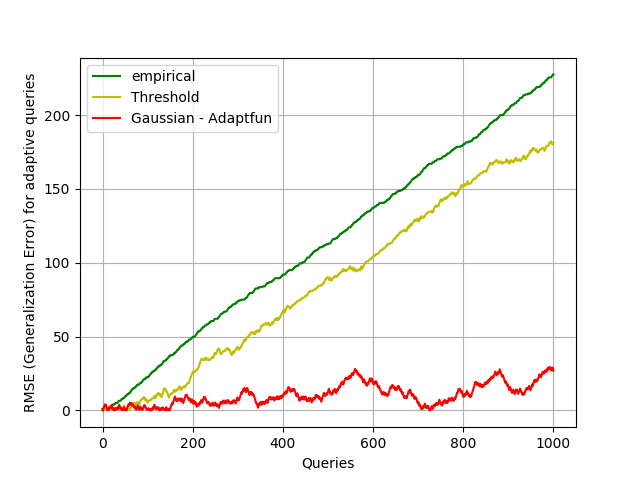
\includegraphics[width=1.0\textwidth]{exp_adaptivity.png}
\caption{}
\end{centering}
\end{subfigure}
\vspace{-0.2cm}
 \caption{The adaptive data analysis programs with
 (a) $O(1)$ adaptivity, 
 (b) $O(n)$ adaptivity,
 (c) and $O(2^n)$ adaptivity.
}
\label{fig:implementation_generalization_errors}
\vspace{-0.6cm}
\end{figure}
}
